\documentclass[11pt,a4paper]{article}

\usepackage[utf8]{inputenc}
\usepackage[T1]{fontenc}
\usepackage[english]{babel}
\usepackage{amsmath,amssymb}
\usepackage{graphicx}
\usepackage{xcolor}
\usepackage{booktabs}
\usepackage{caption}
\usepackage{subcaption}
\usepackage[margin=2.4cm]{geometry}
\usepackage{placeins}
\usepackage{hyperref}
\hypersetup{colorlinks=true,linkcolor=blue!50!black,urlcolor=blue!50!black}
\graphicspath{{figures/}}

% "Part" divider used to separate the two studies
\newcommand{\partbar}[1]{%
  \bigskip
  \begin{center}\large\bfseries #1\end{center}
  \medskip
}

\title{%
\textbf{Development of an Automatic Design Optimization Platform\\
for a 2D Heat-Conduction System Using FreeFEM++}\\[4pt]
\large HEAT-COND benchmark with FreeFEM++ and Python}
\author{Laurent Zhu \and Alexandre Le Droucpeet}
\date{Optimization and Numerical Analysis (MATH6304P-260-M01), Spring 2026\\
Shanghai Jiao Tong University, SPEIT}

\begin{document}
\maketitle

\begin{abstract}
\noindent We develop a compact, automatic design-optimization platform for the 2D
steady-state HEAT-COND heat-conduction benchmark, coupling a FreeFEM++ $P_1$ finite-element
solver with a Python optimization driver. The study is organized in two parts.
\textbf{Part~I} solves the original benchmark: maximizing the mean fin temperature
$J$ over the conductivities and the Biot number. Through systematic studies we show that
this objective is smooth and unimodal with a \emph{boundary} optimum at
$\mathbf{x}^\star=(1,1,1,1,1,0.01)$, giving $J^\star\approx0.730$ at mesh density~50 (an
$\approx850\%$ improvement over the uniform design), and that \textbf{Nelder--Mead} is among the
most efficient optimizers (Bayesian optimization reaches the same optimum in still fewer evaluations). \textbf{Part~II} enriches the problem into
a realistic engineering design: each fin now carries a \emph{discrete material} (conductivity,
price, density) and a \emph{continuous geometry} (thickness, length), and we maximize a
multi-criteria objective $F = Q - \lambda_{\text{cost}}\,\text{Cost} - \lambda_{\text{mass}}\,\text{Mass}$.
On this $16$-dimensional, mixed integer/continuous problem we apply the same methods as in Part~I
together with \textbf{Bayesian optimization}; they land within a few percent, and Bayesian optimization
attains the best objective using by far the fewest evaluations, so we retain it as the default.
We characterize its convergence both per evaluation and in CPU time, and a
performance--cost Pareto sweep shows that the material cost can be cut by about $90\%$ for a
moderate performance loss.
\end{abstract}

\section{Introduction and Project Objective}
This project develops a compact, automatic design-optimization platform for a two-dimensional
steady-state heat-conduction problem, the HEAT-COND benchmark drawn from the reduced-basis
literature~\cite{ballout2024}. The platform integrates, within a single reproducible workflow,
the five required components: a finite-element solver written in FreeFEM++, an objective-evaluation
module, a Python optimization driver, a graphical user interface, and a numerical-analysis
framework for comparing optimization strategies.

The report follows a deliberate two-step structure. \textbf{Part~I} answers the original
benchmark question with the simple objective $J$ (the mean fin temperature) and identifies the
best-suited optimizer \emph{and why}. \textbf{Part~II} then enriches the design space with the
choice of material (with its price and density) and the dimensioning of each fin (thickness and
length), turning the academic benchmark into a genuine multi-objective engineering design and
re-examining which optimization strategy is best on this harder, mixed and non-smooth landscape.
A single structural idea ties the two parts together: the geometry of the objective (smooth and
unimodal versus mixed and non-smooth) dictates which optimizer wins.

\section{Mathematical Model (Initial Problem)}
\subsection{Geometry}
The computational domain $\Omega\subset[0,1]^2$ is a comb-shaped region consisting of a central
vertical \emph{spine} of width $w_s=0.10$ and five pairs of horizontal \emph{fins} of thickness
$t_f=0.06$, centred at $y\in\{0.16,0.32,0.48,0.64,0.80\}$. The inner spine edges are at
$x_g=(1-w_s)/2=0.45$ and $x_d=x_g+w_s=0.55$. Two boundary regions are distinguished:
$\Gamma_{\text{Base}}$, the bottom edge of the spine $\{(x,0):x\in[x_g,x_d]\}$, and
$\Gamma_{\text{Fin}}$, the remainder of $\partial\Omega$ (the spine top, the outer fin tips, and
all fin flanks). The domain, its boundary labels and the $P_1$ mesh are shown in
Fig.~\ref{fig:geom}.

\begin{figure}[htbp]
\centering

\includegraphics[width=0.6\textwidth]{geometry_mesh.png}
\caption{HEAT-COND geometry and $P_1$ mesh (density 25). The red base $\Gamma_{\text{Base}}$
carries the Dirichlet condition $T=1$; the blue boundary $\Gamma_{\text{Fin}}$ carries the Robin
condition. The central spine has conductivity $k=1$; each fin $i$ has conductivity $k_i$.}
\label{fig:geom}
\end{figure}

\subsection{Governing Equation}
The dimensionless temperature $T$ satisfies the steady-state heat-conduction equation with mixed
(Dirichlet--Robin) boundary conditions:
\begin{equation}
\begin{cases}
-\nabla\cdot\big(k(\mathbf{x})\,\nabla T\big)=0 & \text{in }\Omega,\\[2pt]
T=1 & \text{on }\Gamma_{\text{Base}},\\[2pt]
k(\mathbf{x})\,\dfrac{\partial T}{\partial n}+\mathrm{Bi}\,T=0 & \text{on }\Gamma_{\text{Fin}}.
\end{cases}
\end{equation}
The conductivity $k(\mathbf{x})$ is piecewise constant: $k=1$ in the spine, and $k=k_i$
($i=1,\dots,5$) in fin $i$, counted bottom to top. The Biot number $\mathrm{Bi}$ controls the
convective coupling on $\Gamma_{\text{Fin}}$.

\subsection{Objective and Optimization Problem}
The objective is to maximize the average temperature on the fin boundary,
\begin{equation}
J(\mathbf{x})=\frac{1}{|\Gamma_{\text{Fin}}|}\int_{\Gamma_{\text{Fin}}}T\,\mathrm{d}\Gamma,
\end{equation}
over $\mathbf{x}=(k_1,\dots,k_5,\mathrm{Bi})\in\mathbb{R}^6$ with $k_i\in[0.1,1.0]$ and
$\mathrm{Bi}\in[0.01,1.0]$: $\max_{\mathbf{x}}J(\mathbf{x})$ subject to box constraints. Physically,
a high $J$ means the spine transfers the heat injected at the base ($T=1$) efficiently to the
peripheral fin surfaces.

\section{Numerical Formulation and FreeFEM++ Implementation}
\subsection{Mesh Generation}
The mesh is constructed explicitly with FreeFEM's \texttt{buildmesh} rather than by truncating a
background grid, so that element edges align exactly with the geometry. The boundary is described
as a closed, counter-clockwise polyline of 44 segments / 45 points, traversed by a single indexed
\texttt{border}; the number of subdivisions of each segment is proportional to its Euclidean length
times a global density \texttt{meshsize}. Two boundary labels are assigned: \textbf{label~1} for the
base segment (Dirichlet) and \textbf{label~2} for the rest of the boundary (Robin). At density 50 the
mesh contains 1151 vertices and 1760 triangles (419 vertices at density 25).

\subsection{PDE Solver}
\texttt{solver.edp} reads its parameters through \texttt{getARGV}. The weak form is assembled in the
$P_1$ space $V_h$: find $T\in V_h$ with $T=1$ on $\Gamma_{\text{Base}}$ such that, for all test
functions $v$,
\begin{equation}
a(T,v)=\int_\Omega k\,\nabla T\cdot\nabla v\,\mathrm{d}\Omega
+\int_{\Gamma_{\text{Fin}}}\mathrm{Bi}\,T\,v\,\mathrm{d}\Gamma=0.
\end{equation}
The Dirichlet condition is imposed strongly via \texttt{on(1, T = 1)}; the Robin condition enters
naturally as the boundary integral over label~2. The objective
$J=\int_{\Gamma_2}T\,\mathrm{d}\Gamma/\int_{\Gamma_2}1\,\mathrm{d}\Gamma$ is computed inside the
solver and printed to stdout as \texttt{Objective\_J=<value>}, removing intermediate text files.

\subsection{Python Coupling and Verification}
The Python layer drives FreeFEM through \texttt{subprocess}: it caches meshes and parses the
objective from stdout. To verify the implementation, the $P_1$ weak form was re-implemented in pure
NumPy and compared against FreeFEM on identical cached meshes: at density 50 the two solvers agree to
six significant digits at the optimal corner ($J(1,1,1,1,1,0.01)=0.730396$ in both), and the
vertex/triangle counts match exactly. This cross-check validates the operator and the objective.

\partbar{Part~I. Initial problem: maximizing the mean fin temperature $J$}

\section{Optimization Strategy (Part~I)}
The driver wraps every algorithm behind a uniform interface returning a normalized dictionary
(\texttt{best\_J}, \texttt{best\_x}, \texttt{n\_eval}, \texttt{time}, full \texttt{history}); random
methods use a fixed seed. We compare \textbf{four methods}, spanning the main families:
\begin{itemize}
  \item \textbf{Nelder--Mead (NM)}: local, deterministic simplex in dimension 6, gradient-free,
  sensitive to the start, very cheap.
  \item \textbf{Differential Evolution (DE)}: global, population-based, gradient-free, robust but
  the most expensive.
  \item \textbf{Adam $\rightarrow$ L-BFGS-B}: a two-phase gradient hybrid, Adam (finite-difference
  gradient, per-coordinate adaptive step) drives the iterate into a good region, then L-BFGS-B
  refines with native bound handling.
  \item \textbf{Bayesian optimization (BO)}: a surrogate-based global method (Gaussian-process model
  with Expected Improvement) aimed at reaching the optimum in as few expensive evaluations as possible;
  it handles the discrete materials of Part~II natively as integer dimensions.
\end{itemize}
Because the objective is a black-box PDE solve, the gradient phase uses central finite differences,
costing $2\times6=12$ extra evaluations per gradient in 6D. The experimental design is implemented as several self-contained studies.

\section{Numerical Results for the Initial Problem}
The reference initial design is $\mathbf{x}_0=(0.5,\dots,0.5)$, for which $J_0\approx0.077$.
Unless stated otherwise, comparisons use mesh density~25; the ranking is identical at density~50.

\subsection{Comparison of the Methods and the Optimal Design}
\begin{table}[h]
\centering
\caption{Comparison of the methods from the common start $\mathbf{x}_0=0.5$ (density 25).}
\begin{tabular}{lrrrl}
\toprule
Method & $J^\star$ & $n_{\text{eval}}$ & Time (s) & Design $\mathbf{x}^\star$\\
\midrule
\textbf{Nelder--Mead} & \textbf{0.73410} & \textbf{90} & 0.16 & $(1,1,1,1,1,0.01)$\\
Adam $\rightarrow$ L-BFGS & 0.73410 & 367 & 0.66 & $(1,1,1,1,1,0.01)$\\
Differential Evolution & 0.72068 & 468 & 0.81 & $(0.80,0.66,0.58,0.62,0.46,0.01)$\\
Bayesian opt. & 0.73410 & 60 & 0.2 & $(1,1,1,1,1,0.01)$\\
\bottomrule
\end{tabular}
\end{table}

Three of the four methods reach the global optimum $\mathbf{x}^\star=(1,1,1,1,1,0.01)$, a vertex of
the admissible box (all conductivities at their upper bound, the Biot number at its lower bound), giving
$J^\star\approx0.730$ at density 50, an $\approx850\%$ improvement over $J_0$; only Differential Evolution
stops short at $J\approx0.721$ with a non-uniform design, its population budget being too small here.
When several methods reach the \emph{same} optimum, what distinguishes them is the \emph{cost} of getting
there. We measure that cost by the number of objective evaluations, because each evaluation is one PDE
solve, the expensive operation; for Nelder--Mead, the gradient hybrid and Differential Evolution this
count is essentially proportional to wall-clock time. By that measure Bayesian optimization is the most
efficient, reaching the corner in only $60$ evaluations against $90$ for Nelder--Mead and $367$ for the
hybrid (Fig.~\ref{fig:e1}). The one caveat is that Bayesian optimization also fits a surrogate at each
step; this overhead is negligible against a true FreeFEM solve but not against the very fast NumPy
reference solver, so its real advantage lies in the expensive evaluations it saves. The effect on the
temperature field is shown in Fig.~\ref{fig:tfields}: the initially cold fins ($T$ down to $0.003$ at the
tips) become hot ($T\ge0.601$).

\begin{figure}[htbp]
\centering
\begin{subfigure}{0.56\textwidth}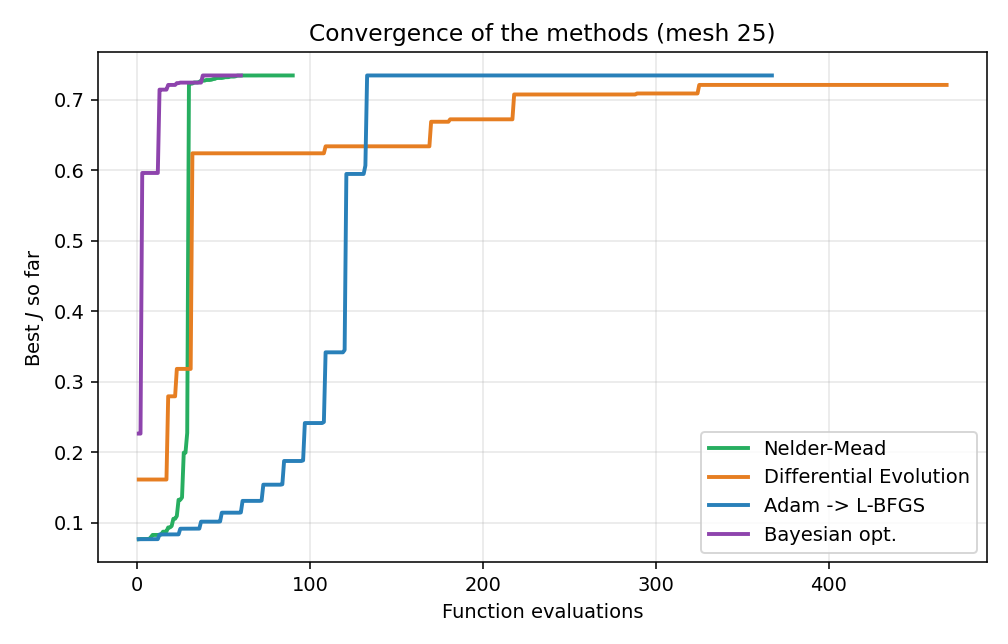
\includegraphics[width=\linewidth]{part1_methods_convergence.png}\end{subfigure}
\hfill
\begin{subfigure}{0.42\textwidth}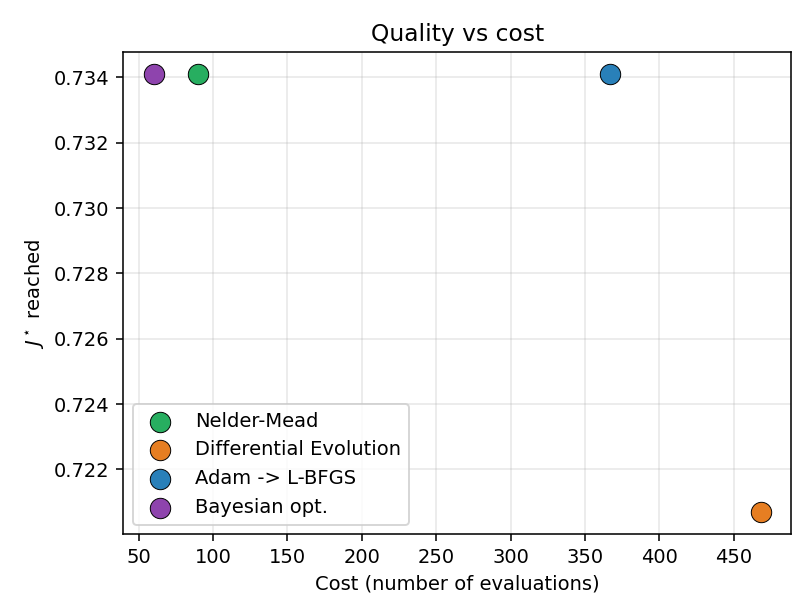
\includegraphics[width=\linewidth]{part1_quality_vs_cost.png}\end{subfigure}
\caption{Convergence (left) and quality-vs-cost trade-off (right). Nelder--Mead and the gradient
hybrid reach the optimal corner (Nelder--Mead in the fewest evaluations); Differential Evolution falls
short at this budget, and Bayesian optimization is the most sample-efficient.}
\label{fig:e1}
\end{figure}

\begin{figure}[htbp]
\centering
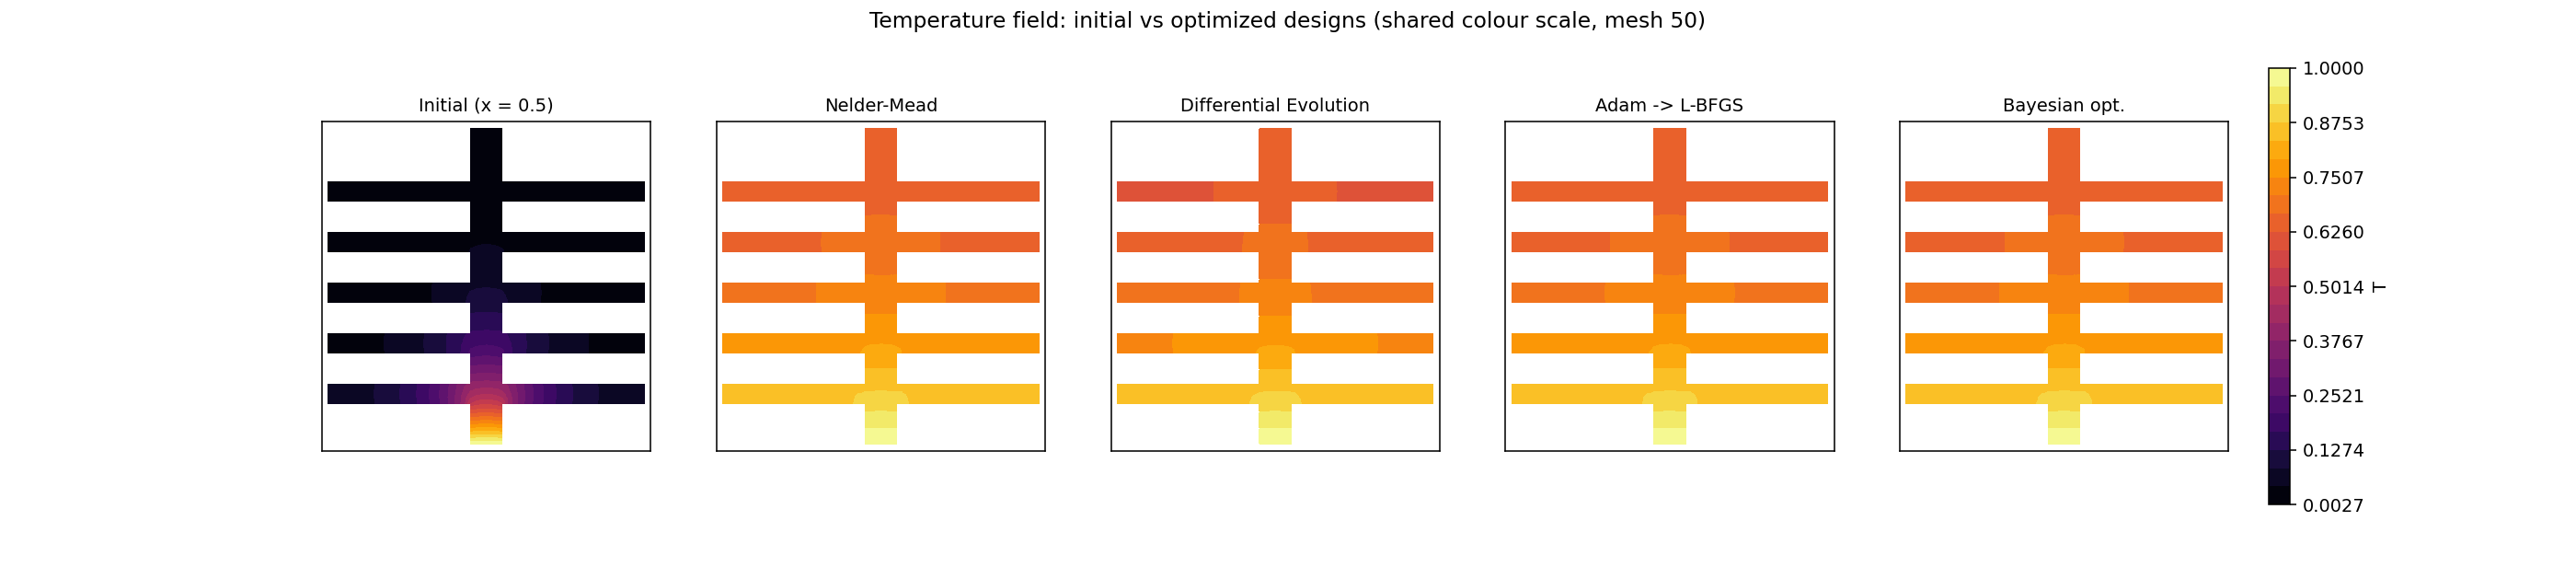
\includegraphics[width=\textwidth]{part1_temperature_fields.png}
\caption{Temperature fields (shared colour scale, mesh 50) for the initial design and the four
optimized designs. Optimization raises the minimum fin temperature from $0.003$ to about $0.60$.}
\label{fig:tfields}
\end{figure}

\subsection{Mesh-Sensitivity}
$J^\star$ decreases monotonically and stabilizes near $0.73$ as the mesh is refined, indicating
approximate mesh-independence by density 50--60; coarse meshes slightly over-estimate the
objective. The wall-clock time grows steeply with density (Fig.~\ref{fig:e2}).

\begin{figure}[htbp]
\centering
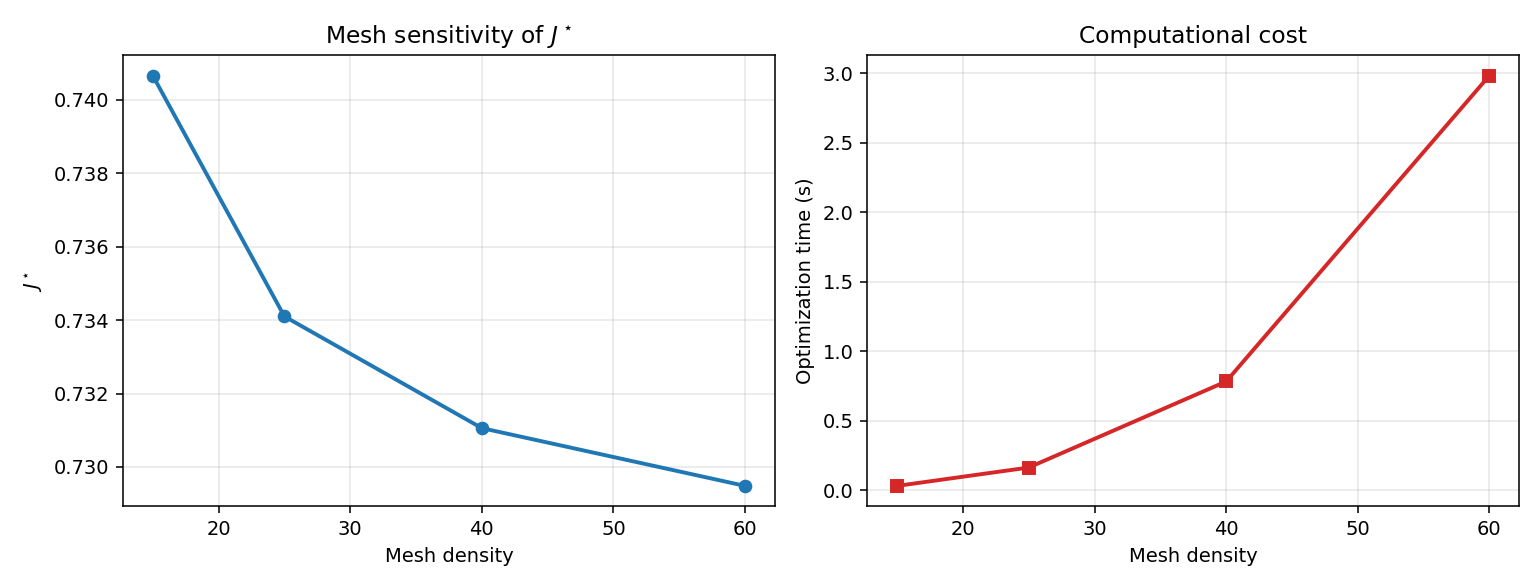
\includegraphics[width=0.9\textwidth]{part1_mesh_sensitivity.png}
\caption{Mesh-sensitivity of $J^\star$ (left) and computational cost (right).}
\label{fig:e2}
\end{figure}

\begin{table}[h]
\centering
\caption{Optimized objective (Nelder--Mead) vs mesh density.}
\begin{tabular}{lcccc}
\toprule
Mesh density & 15 & 25 & 40 & 60\\
\midrule
$J^\star$ & 0.7407 & 0.7341 & 0.7311 & 0.7295\\
\bottomrule
\end{tabular}
\end{table}

\subsection{Robustness}
We vary the starting point for the local and gradient methods (NM, Adam) and the random seed for the
stochastic methods (DE, Bayesian optimization). Nelder--Mead and the Adam$\rightarrow$L-BFGS hybrid reach
the corner from every start; Differential Evolution and Bayesian optimization, being stochastic, show a
small seed-to-seed spread (a few $\times10^{-3}$). The objective is effectively unimodal, so the methods
are highly reproducible (Fig.~\ref{fig:e34}).

\begin{figure}[htbp]
\centering
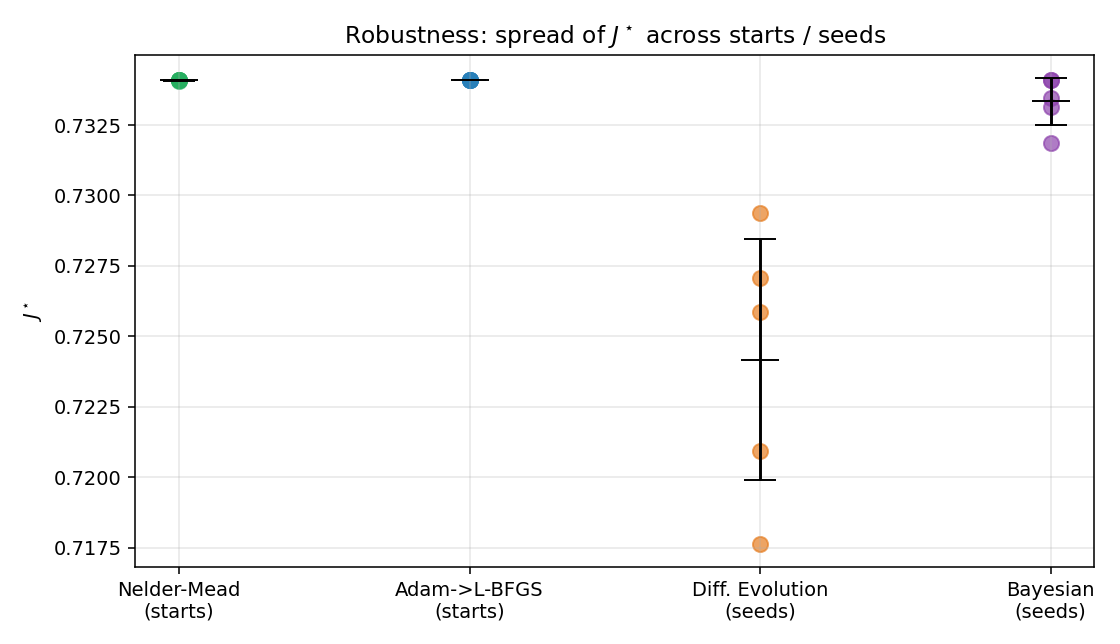
\includegraphics[width=0.85\textwidth]{part1_robustness.png}
\caption{Variability of $J^\star$ across starting points (NM, Adam) and across seeds (DE).}
\label{fig:e34}
\end{figure}

\subsection{Gradient Methods: the Hybrid and its Components}
This study isolates the contribution of each phase by adding two diagnostic runs from
$\mathbf{x}_0=0.5$:
\begin{table}[h]
\centering
\caption{Diagnostic runs of the gradient hybrid (density 25).}
\begin{tabular}{lrrl}
\toprule
Variant & $J^\star$ & $n_{\text{eval}}$ & Reaches the corner\\
\midrule
Adam $\rightarrow$ L-BFGS & 0.734100 & 367 & yes\\
\emph{Adam alone} & 0.734100 & 360 & yes\\
\emph{L-BFGS-B alone} & 0.734100 & 161 & yes\\
\bottomrule
\end{tabular}
\end{table}

All three gradient variants reach the corner. On this smooth reference solver, scipy's
bound-constrained L-BFGS-B reaches it on its own (161 evaluations), so the Adam warm-start is not
strictly required here; its benefit shows on noisier or more strongly ill-conditioned objectives, where
a pure quasi-Newton step can stall. The objective is markedly ill-scaled: the gradient in the Biot
direction dominates those in the conductivity directions, yet the box constraints and the smoothness let
the quasi-Newton iterates slide to the corner. Adam contributes the complementary idea of per-coordinate
adaptive steps, which normalize this imbalance and make the hybrid robust. Nelder--Mead and the gradient
methods converge to the same physical design; Differential Evolution, short of budget, does not
(Fig.~\ref{fig:designs}).

\begin{figure}[htbp]
\centering
\begin{subfigure}{0.56\textwidth}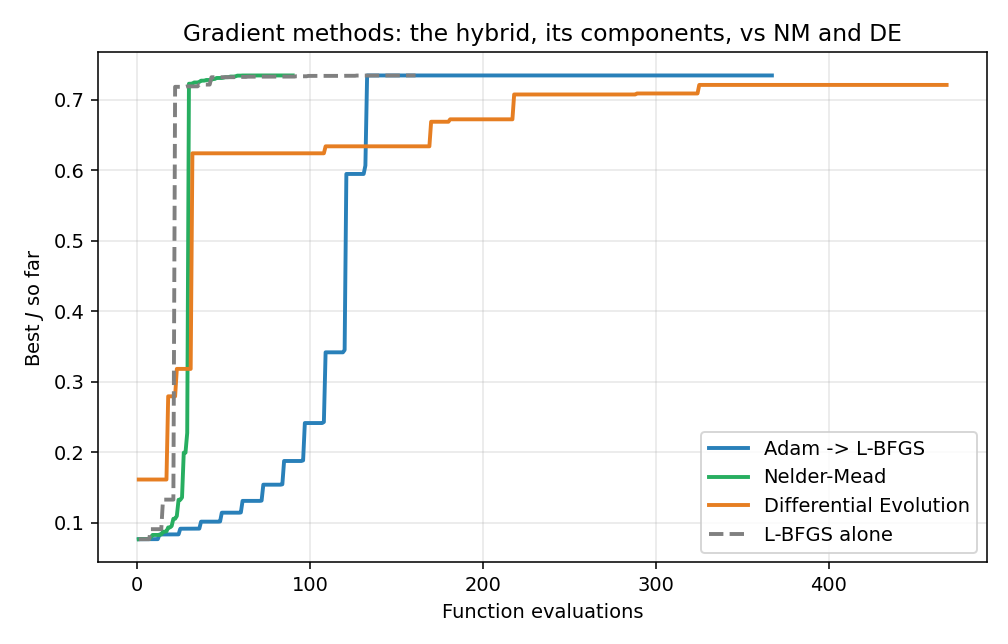
\includegraphics[width=\linewidth]{part1_gradient_methods.png}\caption{}\label{fig:e7}\end{subfigure}
\hfill
\begin{subfigure}{0.42\textwidth}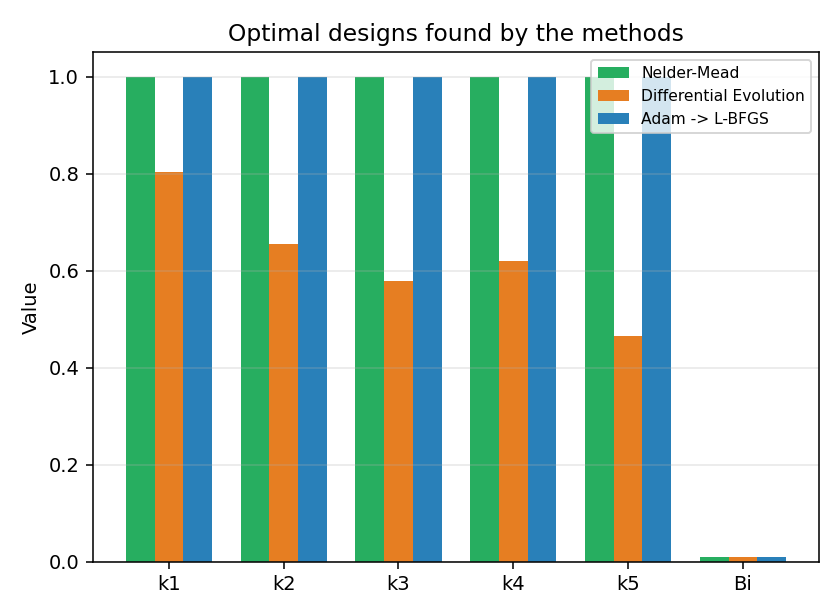
\includegraphics[width=\linewidth]{part1_optimal_designs.png}\caption{}\label{fig:designs}\end{subfigure}
\caption{(a) Convergence of the hybrid against NM and DE, and of L-BFGS-B alone (dashed), which also
reaches the optimum. (b) Optimal designs: Nelder--Mead and the gradient methods converge to
$k_i\to1$, $\mathrm{Bi}\to0.01$; Differential Evolution, short of budget, lands on a non-uniform design.}
\end{figure}

\subsection{Conclusion of Part~I}
The initial HEAT-COND objective is \emph{smooth and unimodal with a boundary optimum} at
$\mathbf{x}^\star=(1,1,1,1,1,0.01)$, $J^\star\approx0.730$. On this landscape \textbf{Nelder--Mead is
the most efficient optimizer and the recommended default}; Differential Evolution, given a sufficient
budget, serves as a global-optimality check, and the gradient methods (Adam$\rightarrow$L-BFGS) reach the
optimum efficiently. This corner optimum is, however, an artefact of higher conductivity being free,
which motivates Part~II.

\FloatBarrier
\partbar{Part~II. Enriched problem: material and geometry design (complex objective)}

\section{Enriched Model: Material, Dimensioning and a Multi-Objective Goal}
The Part~I optimum sits at a vertex of the box because raising any conductivity carries no cost. A
realistic design must pay for what it builds. We therefore enrich the problem on two fronts at once:
each fin is assigned a \emph{discrete material} (fixing its conductivity, price and density) and a
\emph{continuous geometry} (thickness and length, which physically reshape the mesh).

\subsection{Design Vector and Material Catalogue}
The design becomes 16-dimensional, grouped by type,
\begin{equation}
\mathbf{x}=[\,m_1\dots m_5\ \mid\ t_1\dots t_5\ \mid\ \ell_1\dots\ell_5\ \mid\ \mathrm{Bi}\,],
\end{equation}
where $m_i\in\{0,1,2,3\}$ selects fin $i$'s material from the catalogue of Table~\ref{tab:mat},
$t_i\in[0.02,0.14]$ is its thickness, $\ell_i\in[0.10,0.45]$ its length, and $\mathrm{Bi}\in[0.01,1]$.
The five $m_i$ are \emph{integer} variables; the eleven remaining variables are continuous.

\begin{table}[h]
\centering
\caption{Material catalogue (illustrative, normalized values). The index $m_i$ fixes a fin's
conductivity $k$, unit price and density.}
\label{tab:mat}
\begin{tabular}{clccc}
\toprule
Index & Material & $k$ & Price/vol. & Density\\
\midrule
0 & Copper    & 1.00 & 9.0 & 9.0\\
1 & Aluminium & 0.60 & 3.0 & 2.7\\
2 & Steel     & 0.25 & 1.5 & 7.8\\
3 & Polymer   & 0.05 & 0.3 & 1.2\\
\bottomrule
\end{tabular}
\end{table}

\subsection{Objective: Heat Dissipated versus Cost and Mass}
We maximize the scalarized objective
\begin{equation}
F(\mathbf{x}) = Q(\mathbf{x})
 - \lambda_{\text{cost}}\sum_{i=1}^{5}\text{price}(m_i)\,A_i
 - \lambda_{\text{mass}}\sum_{i=1}^{5}\text{density}(m_i)\,A_i,
\qquad A_i = 2\,t_i\,\ell_i,
\end{equation}
where $A_i$ is the area of fin pair $i$ (left+right symmetric) and the performance is the
\emph{heat dissipated through the fins},
\begin{equation}
Q(\mathbf{x})=\int_{\Gamma_{\text{Fin}}}\mathrm{Bi}\,T\,\mathrm{d}\Gamma .
\end{equation}
We deliberately use $Q$ rather than the Part~I mean temperature $J$. Indeed $J$ \emph{increases} as
fins shrink (less lossy surface), which would align performance with low cost and \emph{collapse} the
trade-off into a degenerate front. The dissipated heat $Q$ instead grows with surface, conductivity
and Biot number, so it genuinely \emph{opposes} cost and mass. Throughout
Part~II we use $\lambda_{\text{cost}}=0.05$ and $\lambda_{\text{mass}}=0.02$ unless a sweep is stated.

\subsection{Numerical Treatment and Multi-Fidelity}
Because the geometry $(t_i,\ell_i)$ is now part of the design, the mesh must be \emph{regenerated at
every evaluation} (it can no longer be cached once and reused, as in Part~I). To keep the cost
manageable we adopt a \textbf{multi-fidelity} strategy: a global search on a coarse mesh (density
$\sim$18--20), then a local refinement (Nelder--Mead, materials frozen) on a fine mesh (density
$\sim$45--50). Each evaluation's wall-clock time is logged in the run history. To keep the optimizer
comparison fast and fully reproducible, it is run on a validated pure-NumPy reference solver (an
extension to variable geometry of the cross-check solver of Sec.~3.3): at the default geometry it
reproduces the Part~I corner value $J=0.730$ to three digits, so it ranks the methods faithfully
while costing only a few milliseconds per evaluation on the coarse mesh.

\section{Numerical Results for the Enriched Problem}

\subsection{Comparison of the Optimization Methods}
To keep the methodology consistent across the report, we apply to the enriched problem the
\emph{same three optimizers as in Part~I} (Nelder--Mead (NM), Differential Evolution (DE) and the
Adam$\rightarrow$L-BFGS hybrid. The five discrete material variables are handled by \emph{continuous
relaxation with rounding} (the material index is rounded inside the objective), exactly as DE already
treated them in Part~I) together with \textbf{Bayesian optimization}, so all four methods operate on the
same $16$-dimensional continuous box.
Table~\ref{tab:enr-methods} and Fig.~\ref{fig:enr-conv} report the comparison on the coarse mesh (each method run to convergence).

\begin{table}[h]
\centering
\caption{The four optimizers on the enriched problem (coarse mesh, $\lambda_{\text{cost}}=0.05$,
$\lambda_{\text{mass}}=0.02$). $F$ is the maximized objective; $Q$, cost and mass describe the best
design. Times are for the NumPy reference solver.}
\label{tab:enr-methods}
\begin{tabular}{lrrrrrr}
\toprule
Method & $F^\star$ & $Q$ & Cost & Mass & $n_{\text{eval}}$ & Time (s)\\
\midrule
\textbf{Bayesian opt.} & \textbf{0.5687} & 0.6225 & 0.760 & 0.791 & \textbf{80} & 0.1\\
Adam $\rightarrow$ L-BFGS & 0.5667 & 0.5918 & 0.369 & 0.333 & 1045 & 1.2\\
Nelder--Mead & 0.5586 & 0.5899 & 0.436 & 0.474 & 577 & 1.0\\
Differential Evolution & 0.5484 & 0.5983 & 0.612 & 0.966 & 720 & 1.2\\
\bottomrule
\end{tabular}
\end{table}

The four methods land within a few percent of each other ($F^\star=0.548$--$0.569$).
\textbf{Bayesian optimization attains the best objective} ($F^\star=0.5687$), and does so with
\textbf{by far the fewest evaluations} ($80$, against $577$--$1045$ for the others): its Gaussian-process
surrogate spends evaluations where they most improve the objective, and it treats the five materials
natively as integer dimensions. It reaches a high-performance design (the highest dissipated heat,
$Q=0.62$) by placing copper on the hottest bottom fin and accepting a higher material cost; the net
objective still wins. The Adam$\rightarrow$L-BFGS hybrid is a close second ($0.5667$) at a cheaper, lighter
design; Nelder--Mead follows ($0.559$); Differential Evolution trails ($0.548$), again needing a larger
budget while still serving as a \emph{global} check. \textbf{We therefore retain Bayesian optimization}
as the default method for the detailed studies below: it gives both the best objective and, decisively
when each evaluation is an expensive PDE solve, the fewest evaluations.

\begin{figure}[htbp]
\centering
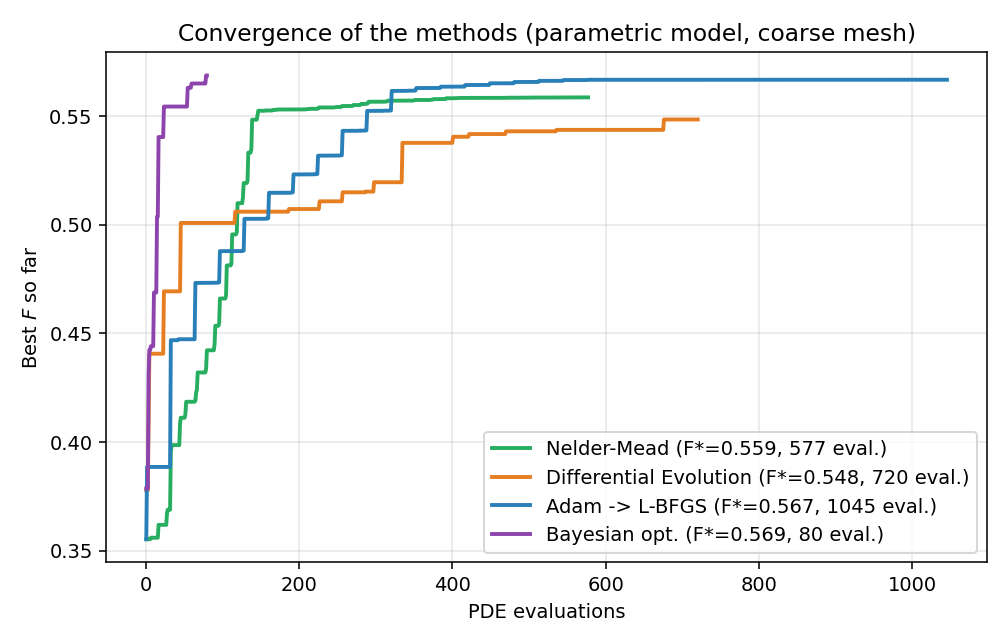
\includegraphics[width=0.66\textwidth]{part2_methods_convergence.png}
\caption{Best-so-far objective $F$ versus PDE evaluations for the four methods (coarse mesh). Bayesian
optimization reaches the highest objective in by far the fewest evaluations; the Adam$\rightarrow$L-BFGS
hybrid is a close second.}
\label{fig:enr-conv}
\end{figure}

\subsection{The Optimal Enriched Design}
Figure~\ref{fig:enr-diag} traces the retained run: the objective and its best-so-far envelope, and the
joint evolution of the best design's performance $Q$, cost and mass. The optimal design
(Fig.~\ref{fig:enr-design}) places \emph{copper}, the most conductive material, on the large bottom
fin ($t=0.14$, $\ell=0.27$), where the temperature and hence the marginal heat transfer are highest; the
upper fins use cheaper aluminium, steel and polymer, and the Biot number saturates at its upper bound
($\mathrm{Bi}=1.0$, which maximizes the dissipated heat $Q=\int \mathrm{Bi}\,T$). Spending the costly
material exactly where it pays off yields the highest performance of all methods ($Q=0.62$) at a moderate
cost ($0.76$), and the best objective of the comparison ($F=0.569$).

\begin{figure}[htbp]
\centering
\begin{subfigure}{0.52\textwidth}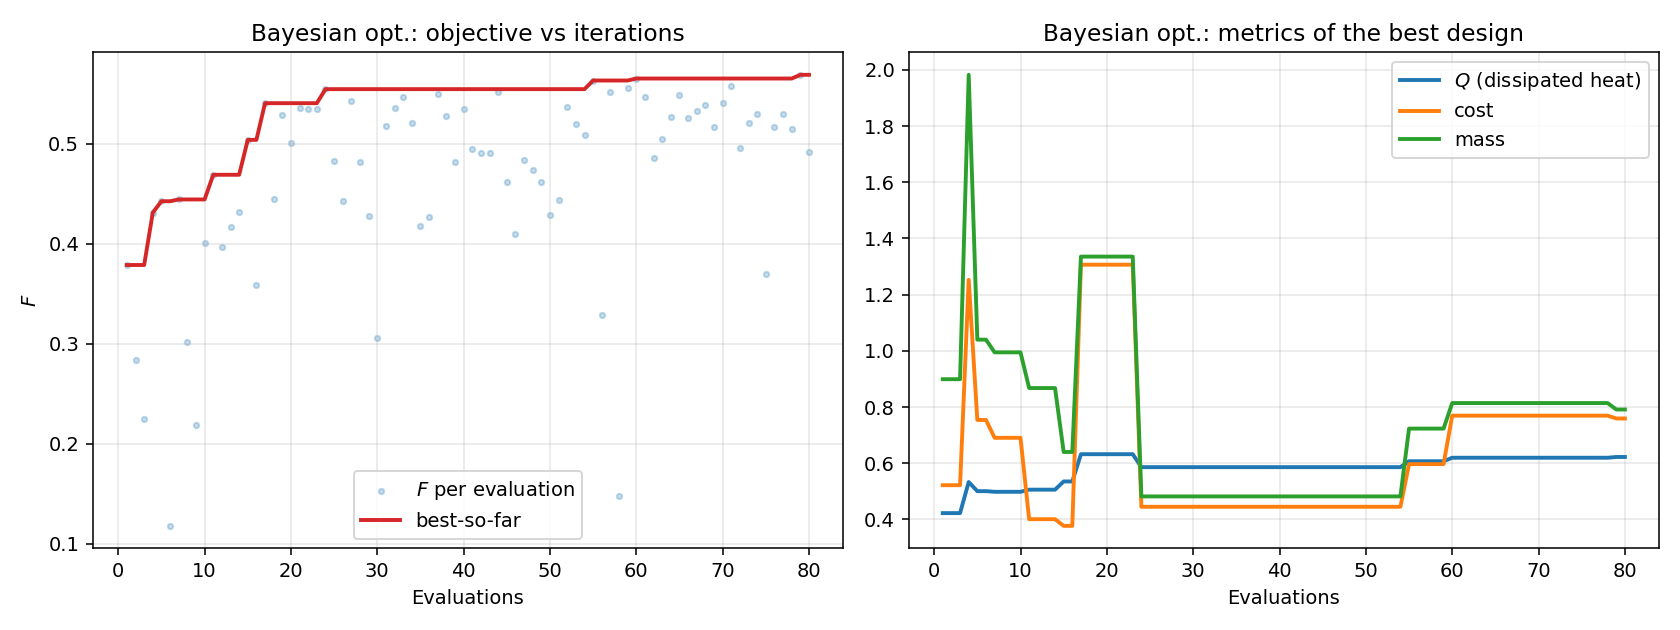
\includegraphics[width=\linewidth]{part2_best_diagnostics.png}\caption{}\label{fig:enr-diag}\end{subfigure}
\hfill
\begin{subfigure}{0.46\textwidth}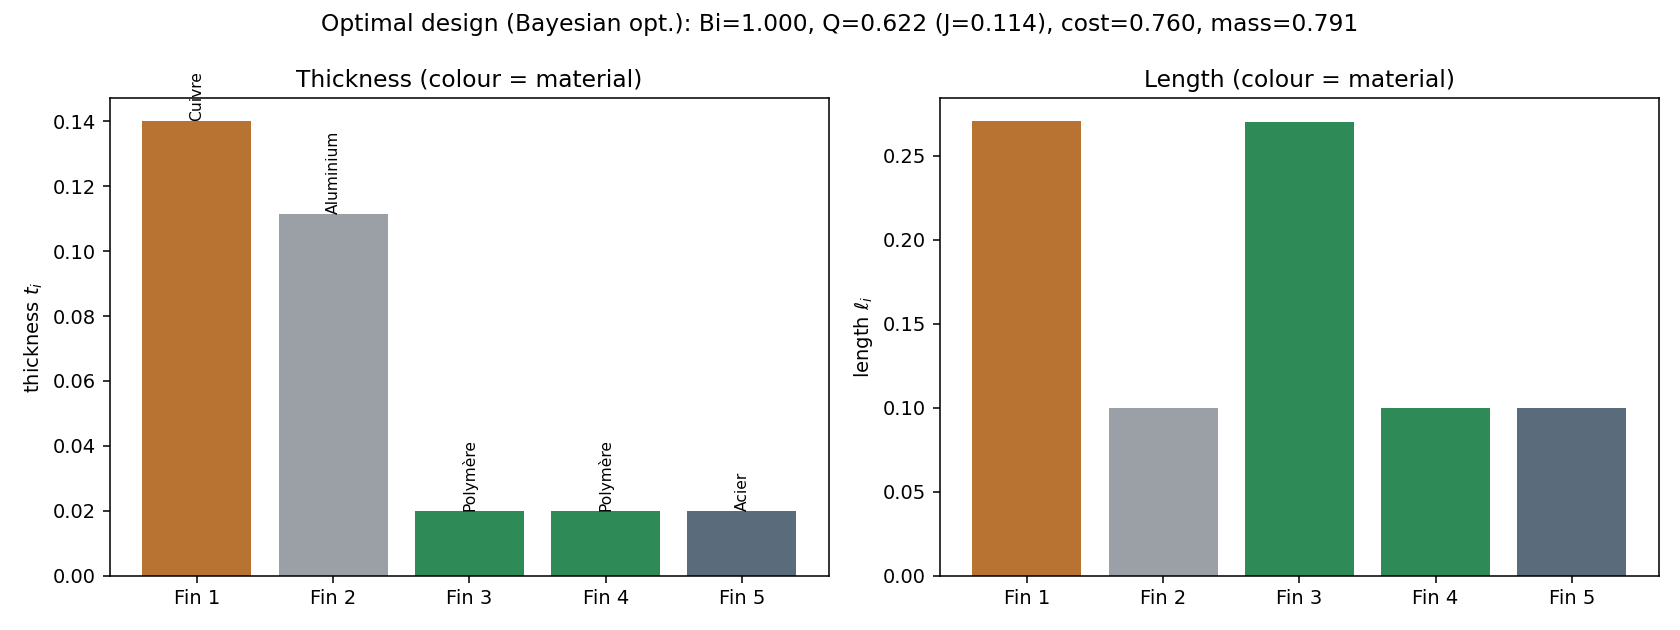
\includegraphics[width=\linewidth]{part2_optimal_design.png}\caption{}\label{fig:enr-design}\end{subfigure}
\caption{Retained method (Bayesian optimization). (a)~Objective per evaluation with best-so-far
envelope, and the performance/cost/mass of the running-best design. (b)~Composition of the optimal
design: thickness and length per fin, coloured by material (copper on the bottom fin).}
\end{figure}

\subsection{Evolution of the Objective for the Retained Method}
Having selected Bayesian optimization, we characterize how its objective improves, both
\emph{per evaluation} and \emph{in CPU time} (Fig.~\ref{fig:enr-evo}). The run reaches $F^\star=0.569$
in only $80$ evaluations: most of the gain comes in the first dozen surrogate-guided steps, after which
the curve flattens, a clear diminishing-returns plateau and a natural stopping point. This is the sample
efficiency that motivates a surrogate method on an expensive objective; the Gaussian-process fitting adds
a little per-iteration overhead, negligible next to a FreeFEM PDE solve.

\begin{figure}[htbp]
\centering
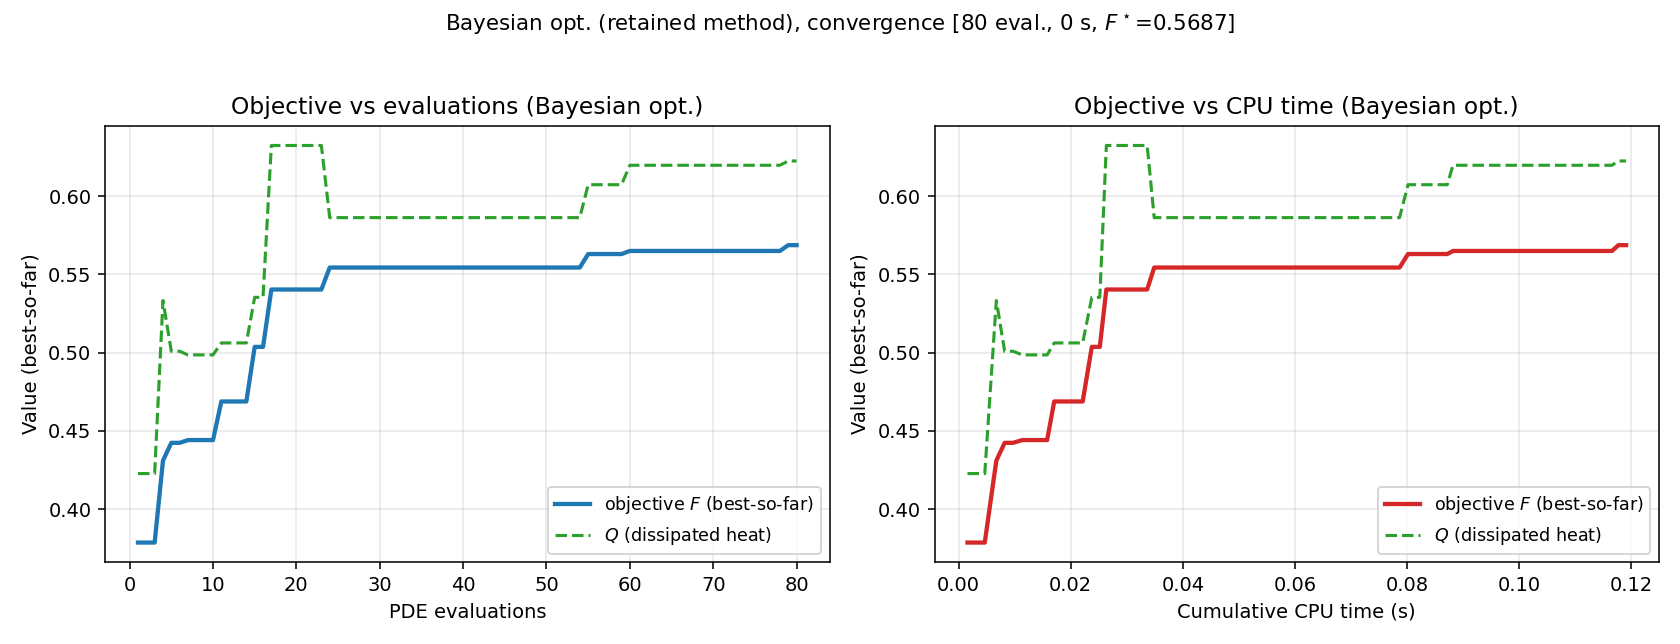
\includegraphics[width=\textwidth]{part2_objective_evolution.png}
\caption{Convergence of the retained method (Bayesian optimization): best-so-far objective $F$ (and
the performance $Q$) versus the number of PDE evaluations (left) and versus cumulative CPU time
(right).}
\label{fig:enr-evo}
\end{figure}

\subsection{Performance--Cost Pareto Front}
To expose the full trade-off we sweep the cost weight $\lambda_{\text{cost}}$ and re-optimize with the
retained method for each value, tracing the performance--cost Pareto front (Table~\ref{tab:pareto},
Fig.~\ref{fig:enr-pareto}). As $\lambda_{\text{cost}}$ grows, the optimizer trades performance for
economy in a strongly concave way: from $\lambda=0$ to $\lambda=0.20$ the material cost drops by about
$91\%$ ($1.21\to0.11$) for a $\approx15\%$ loss of performance $Q$ ($0.63\to0.54$). The knee near
$\lambda\approx0.05$--$0.10$ removes most of the cost for a modest performance loss.
This turns the otherwise trivial Part~I corner problem into a genuine multi-objective design study with
an exploitable front.

\begin{table}[h]
\centering
\caption{Pareto sweep (retained method, coarse mesh): performance $Q$, material cost and mass of the
optimal design versus the cost weight $\lambda_{\text{cost}}$ (with $\lambda_{\text{mass}}=0.02$).}
\label{tab:pareto}
\begin{tabular}{rrrrr}
\toprule
$\lambda_{\text{cost}}$ & $Q$ & Cost & Mass & $F$\\
\midrule
0.00 & 0.6323 & 1.213 & 1.235 & 0.6076\\
0.02 & 0.6321 & 1.174 & 1.184 & 0.5850\\
0.05 & 0.6225 & 0.760 & 0.791 & 0.5687\\
0.10 & 0.6027 & 0.572 & 0.614 & 0.5333\\
0.20 & 0.5353 & 0.107 & 0.157 & 0.5108\\
\bottomrule
\end{tabular}
\end{table}

\begin{figure}[htbp]
\centering
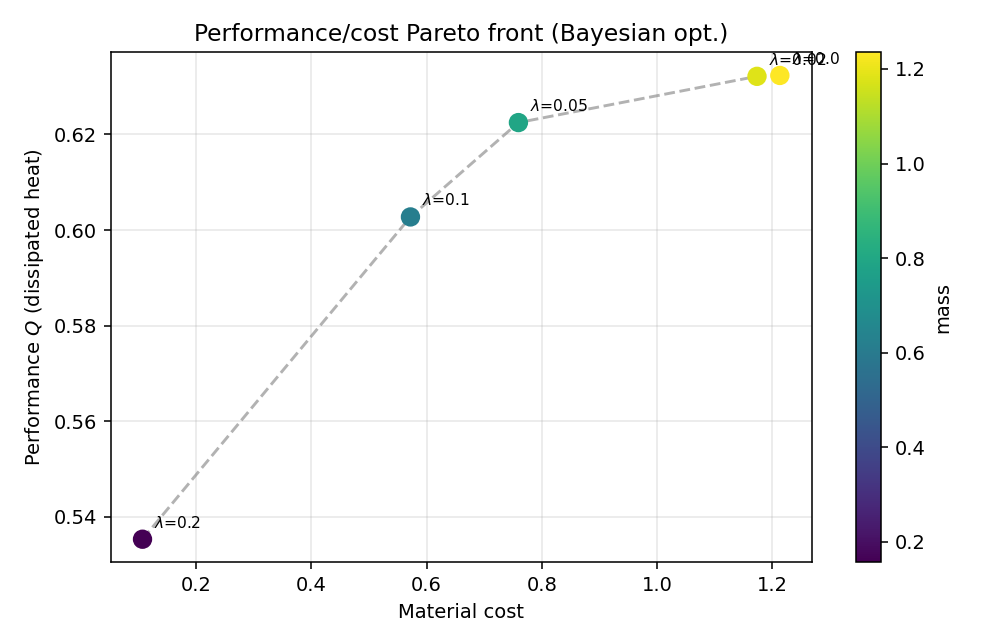
\includegraphics[width=0.66\textwidth]{part2_pareto_front.png}
\caption{Performance--cost Pareto front of the enriched problem (colour = mass). Each point is an
optimum for a given cost weight $\lambda_{\text{cost}}$; the front is strongly concave near the
high-performance end.}
\label{fig:enr-pareto}
\end{figure}

\subsection{Multi-Fidelity Cost Control}
Because the mesh is rebuilt at every evaluation, a fine mesh is accurate but costly, so the idea is to
spend the bulk of the search budget on a cheap coarse mesh and only a few evaluations on the accurate
fine mesh. The pipeline is a \emph{global-then-local} split across mesh fidelities: a global method on
the coarse mesh, then a local method on the fine mesh with the materials frozen so only the continuous
geometry is polished.

The choice of optimizer at each stage is dictated by the stage, not by which method won the
single-fidelity comparison. One might expect to reuse Bayesian optimization (the retained method of
Section~7.1) and L-BFGS-B here, but neither fits its stage. Bayesian optimization is valuable precisely
when each evaluation is \emph{expensive}: it spends real compute fitting a Gaussian-process surrogate to
save evaluations. On the coarse mesh an evaluation costs only a few milliseconds, so the surrogate
overhead is no longer amortized, and Bayesian optimization would be slower in wall-clock time than a
plain population search for the same number of solves. We therefore use Differential Evolution for the
global stage: it is cheap per step, explores the discrete materials broadly, and needs no starting
point. For the fine stage we use Nelder--Mead rather than L-BFGS-B (or the Adam$\rightarrow$L-BFGS
hybrid) because remeshing makes the fine-mesh objective slightly non-smooth, which corrupts the
finite-difference gradient those methods rely on; a gradient-free local search is more robust to that
noise. In short, Bayesian~$+$~L-BFGS is the right pairing for a single expensive fidelity, whereas
DE~$+$~Nelder--Mead is the right pairing once the two-fidelity split has made the global stage cheap and
the local stage noisy.

Figure~\ref{fig:enr-mf} shows the pipeline: a coarse-mesh global search (Differential Evolution, $448$
evaluations) followed by a fine-mesh local refinement (Nelder--Mead, density~45, $173$ evaluations). The
refinement confirms the design; its slightly lower $F$ reflects the fine mesh evaluating $Q$ more
accurately (the coarse mesh over-estimates it, exactly as in the Part~I mesh study). Without this
two-stage strategy, a direct search on the fine mesh would multiply the per-evaluation cost several-fold
for no change in the located optimum.

\begin{figure}[htbp]
\centering
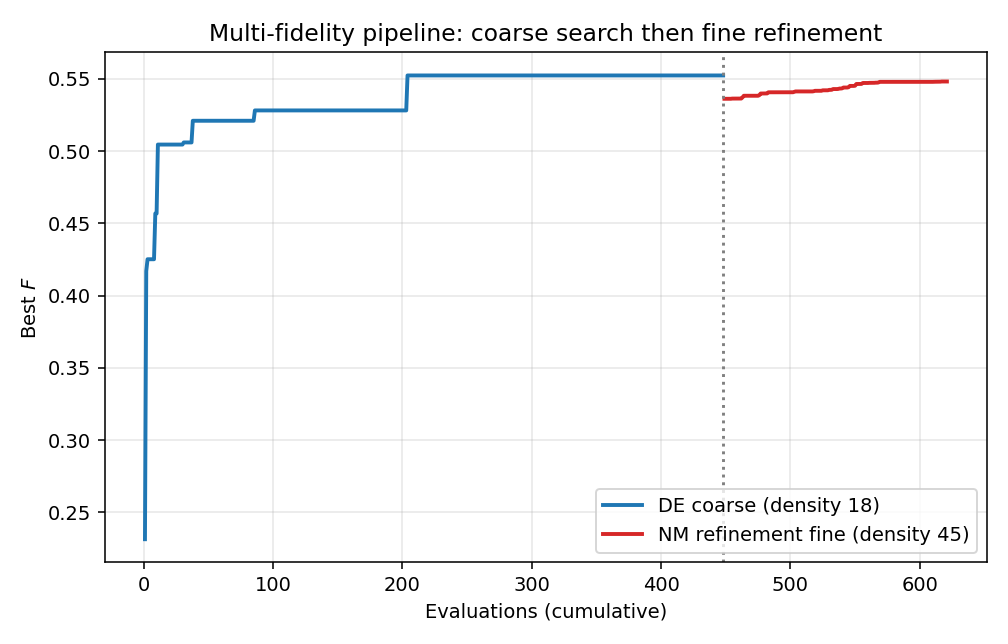
\includegraphics[width=0.66\textwidth]{part2_multifidelity.png}
\caption{Multi-fidelity pipeline: coarse-mesh global search (DE) followed by fine-mesh local
refinement (Nelder--Mead); cumulative evaluations on the horizontal axis, the dotted line marks the
hand-off.}
\label{fig:enr-mf}
\end{figure}

\FloatBarrier
\section{Analysis and Discussion}
\textbf{Two problems, two regimes.} The methodological lesson is that the \emph{same} set of optimizers
behave very differently depending on the landscape. In Part~I the objective is smooth and unimodal with
a boundary optimum, and Nelder--Mead slides straight to the corner, the clear winner: cheapest, most
accurate, most reproducible. In Part~II the objective is $16$-dimensional and mixed (discrete materials)
yet \emph{dominated by its continuous geometry}: the four methods perform within a few percent, and
\emph{Bayesian optimization} attains the best objective using the fewest evaluations, the
Adam$\rightarrow$L-BFGS hybrid a close second, then Nelder--Mead and Differential Evolution. The surrogate
pays off precisely because each evaluation is expensive; the gradient methods stay strong, and
Differential Evolution keeps its role as a global-optimality check. Same platform, same methods: the
ranking tightens and shifts as the landscape changes.

\textbf{Physical reading.} Part~I says ``make everything as conductive as possible and lose as little
heat as possible'' (a corner). Part~II, by pricing material and rewarding dissipated heat, says
something an engineer would recognize: concentrate good material and surface where the temperature is
highest (the lower fins), economize elsewhere, and let the Biot number rise to shed heat. The optimal
design is non-uniform and graded, and the Pareto front quantifies exactly how much performance each
saved unit of material costs.

\textbf{Cost and bottlenecks.} The dominant cost is the FreeFEM PDE solve invoked through a
subprocess. In Part~II the mesh regeneration per evaluation adds to this, which is why the
multi-fidelity split and a bounded evaluation budget matter. Two further levers reduce it: a
surrogate-based search, examined next, and, for the smooth Part~I sub-problem, an analytical/adjoint
gradient.

\textbf{Sample efficiency and Bayesian optimization.} Because every evaluation is an expensive PDE
solve, the currency that matters most is the number of evaluations spent, not wall-clock time alone.
Bayesian optimization targets this directly: it fits a Gaussian-process surrogate to the points already
evaluated and chooses each next point by Expected Improvement, and it handles the discrete materials
natively through integer dimensions. In both parts it is the most sample-efficient method, making most
of its progress in its first evaluations (Figs.~\ref{fig:e1} and~\ref{fig:enr-conv}). Here it does more
than save evaluations: in Part~II it attains the \emph{best} objective ($F=0.569$) using only $80$
evaluations, so it is the retained default; in Part~I it reaches the optimal corner in the fewest
evaluations as well. Bayesian optimization is therefore the recommended method for the expensive
parametric problem, where the number of PDE solves is the binding constraint.

\section{Conclusion and Possible Improvements}
We built an automatic design-optimization platform for HEAT-COND satisfying all required tasks: a
geometry-aligned FreeFEM++ $P_1$ solver, an in-solver objective module, an optimization driver, a
graphical interface and command-line pipeline, and a structured numerical analysis. We then went
beyond the required scope with a fully enriched, multi-objective design problem.

\textbf{Part~I} establishes that the benchmark objective is smooth and unimodal with a boundary optimum
$\mathbf{x}^\star=(1,1,1,1,1,0.01)$, $J^\star\approx0.730$, on which Nelder--Mead is the most efficient
optimizer. \textbf{Part~II} enriches the design with material choice (price, density) and fin
dimensioning, maximizing a performance/cost/mass objective. Applying the same methods plus Bayesian optimization, the four perform within a few percent on this
$16$-dimensional problem, and \textbf{Bayesian optimization attains the best objective using by far the
fewest evaluations}, so it is retained as the default; its convergence is well behaved both per evaluation
and in CPU time, and the performance--cost Pareto front shows the material cost can be cut by about $90\%$
for a moderate performance loss. The other three methods stay within a few percent, the
Adam$\rightarrow$L-BFGS hybrid a close second.

Possible improvements include: (i)~scaling the Bayesian-optimization study demonstrated here to mixed-variable,
higher-dimensional surrogates, to further cut the number of PDE solves; (ii)~an \emph{adjoint gradient} for the
smooth Part~I sub-problem, which would make a gradient method the cheapest option; and (iii)~a richer
material catalogue and manufacturing constraints to bring the enriched problem closer to a real
heat-sink design.

\section*{Member Contributions}
Alexandre Le Droucpeet built the geometry and meshing (the FreeFEM++ \texttt{mesh.edp} and
\texttt{mesh\_param.edp}, and the comb-domain construction) and implemented the optimization methods.
Laurent Zhu carried out the comparative studies of the methods and built the graphical interface.
Both authors wrote the report.

\begin{thebibliography}{1}
\bibitem{ballout2024} H.~Ballout, Y.~Maday, C.~Prud'homme.
\emph{Nonlinear compressive reduced basis approximation for multi-parameter elliptic problem}.
In \emph{Multiscale, Nonlinear and Adaptive Approximation II}, pp.~55--73. Springer, 2024.
\end{thebibliography}

\end{document}
